\documentclass{article}
\usepackage{graphicx}

\title{Analysis of Multithreaded Performance of a Matrix Multiplication Algorithm}
\author{Samuel Wehunt}
\date{\today}

\begin{document}

\maketitle

\section{Problem Definition}
This paper intends to test the performance of a matrix multiplication algorithm
in both serial and multithreaded environments. The purpose of this test is to
calculate the speedup gained by utilising multiple processors, and to test the
efficiency of doing so.
\subsection{Algorithm}
The algorithm chosen for this experiment will be a simple method of calculating
the product of multplying two matrices together. The specific process for this
algorithm can be readily found online, so that will be left as an excercise to
the reader.\\
What is important about this algorithm is that it has a time complexity of $O(n^3)$,
and this property makes it scale very poorly to large problem sets. Another property
of this problem is that it is performed on easily divisible, known-sized data. A third
point about this problem is that no part of the calculation relies on the result of
any other calculation. These aspects make it a nice candidate for parallelization, and
it is hoped that in these tests massive performance gains will be achieved.
\subsection{Test Conditions}
This test will make use of c code that utilizes the OpenMP library for multithreading.
This code assumes square matrices (for simplicity sake; this is not a strict requirement)
and the sizes used for each test will be 1000x1000, 2000x2000, 5000x5000, 7000x7000, and
10000x10000. Each of these problem sets will be executed with 1, 2, 4, 8, 16, and 28 threads.
This process will be repeated twice, so in total there will be 60 executions of the program.
\section{Process}
The conditions of the test are spelled out above. The process for achieving this test will
involve the main c program, and several other auxillary programs to process and present the data.
The program will be run on Tennessee Tech's HPC cluster (more information on that environment below)
through the Slurm batch queuing system. In order to queue up 60 jobs in an efficient manner, a bash
script was written which can iterate through each test case and queue a separate job with the 
necessary hardware resources allocated to it.\\
After the tests have completed, another script (this time written in python), will collect the 
data and plot it on a graph using matplotlib. From that data one can also calculate things such as
the speedup and efficiency of using multiple threads.
\subsection{Test Environment}
My personal computer is not powerful enough to run this problem with the required hardware resources.
Maybe it could do most of the test runs resonably, but it is bogged down by the operating 
system and other programs running on it such as web browsers, chat programs, and video games.
In order to get a proper test this project will be utilising Tennessee Tech's HPC cluster. This
cluster uses the Slurm batch queueing system in order to run jobs from many different users.\\
This cluster also boasts some impressive hardware capabilities. The cluster is made up of 40
non-GPU nodes, and 4 GPU nodes. Each compute node has 128GB of RAM, 28 Xeon cores, and around
200GB of temporary disk storage. Each compute node also has a 1GB Ethernet connection for outside
communication, and a high speed 56GB Infiniband network for file server traffic and high performance
computing communication.\\
These hardware specifications should be sufficient for the purposes of this test.

\section{Results}
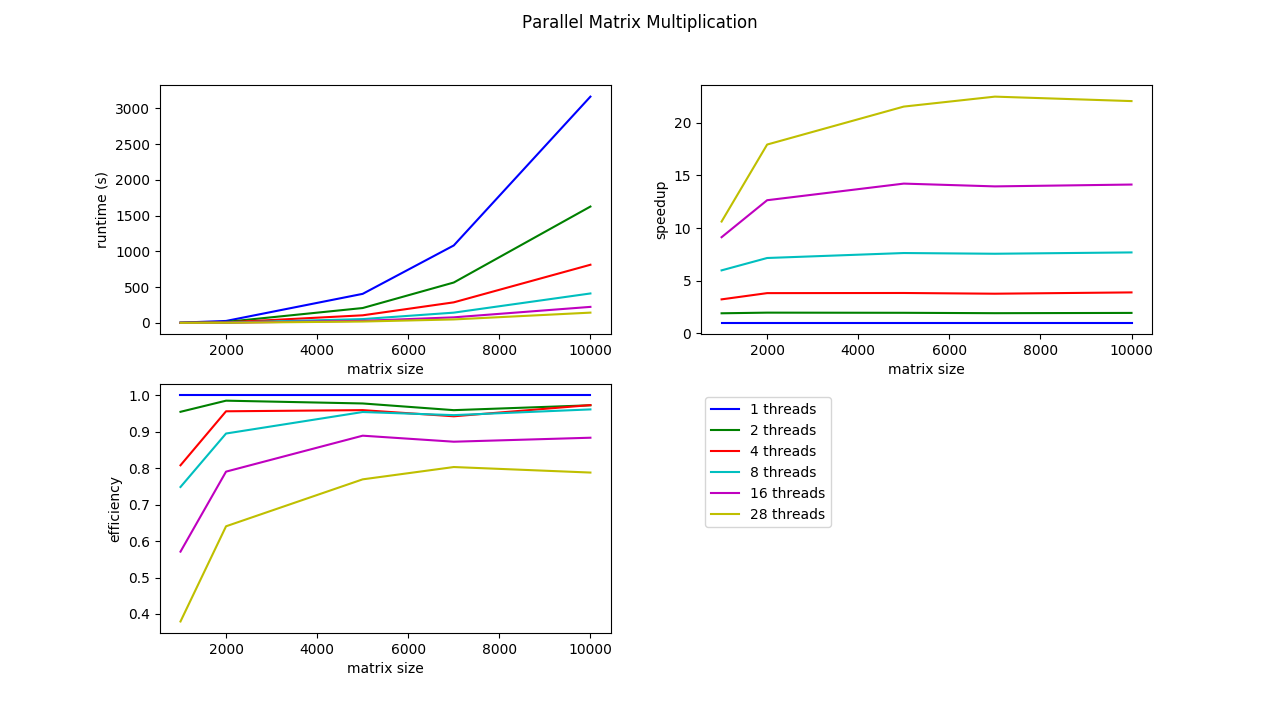
\includegraphics[width=\textwidth]{speedGraph}
All test cases were run and the data was processed as outlined above. Fig 1 shows the execution time
of each run in seconds as opposed to the problem size, Fig 2 shows the speedup 
of each run compared to the single thread execution, and Fig 3 shows the 
efficiency of the multithreaded executions. The results are much what one 
would expect. The problem size corresponds to an exponential growth in run time,
and more threads will cause the algorithm to complete in a shorter amount of time. 
The amount of speedup is also to be expected. The maximum speedup one can achieve
is equal to the amount of threads used, but realistically there is some overhead
in setting up the threads and coordinating the work. The data supports this because
the efficiency is lower as more threads are used. Also when the problem size is small
the efficiency is low, this makes sense because the overhead of setting up threads
still has to happen, and becomes a bigger issue if the problem is small.

\section{Conclusion}
Overall the results of this experiment were not too surprising, and they generally
reflect what was expected. This was a good experiment,and in the future I look forward to
performing more tests where the outcome is not so easily predictable.
\end{document}
